\section{Identification of wave spectrum model}
\subsection{Problem a}
The Power Spectral Density function is the autocorrelation function expressed in the frequency domain. It is formally defined as the Fourier Transform of the autocorrelation function.  The MATLAB function \texttt{pwelch} calculates an estimate of the power spectral density PSD through
dividing the signal into K overlapping blocks multiplied by a windowing function, and finding an
estimate for the periodogram of each one.  The result of sending the waves disturbance, $\psi_w$, through \texttt{pwelch} is shown in \cref{fig:2a-welchPSDestimate}.

\begin{figure}[h]
    \centering
    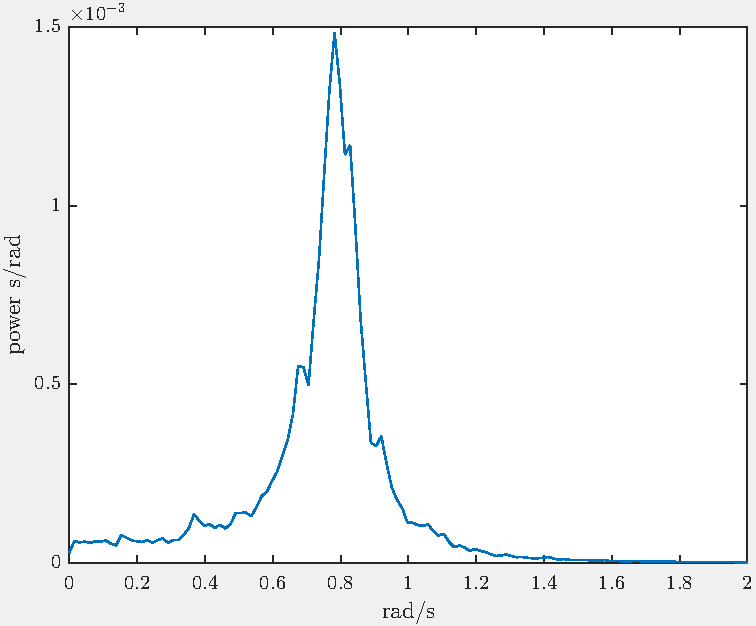
\includegraphics[width=0.5\textwidth]{images/2a-welchPSDestimate}
    \caption{Welch PSD estimate}
    \label{fig:2a-welchPSDestimate}
\end{figure}

\subsection{Problem b}
Using the following state equations in the problem description \cite{assignment}

\begin{align*}
    \xi_w &= \psi_w \\
    \dot{\psi}_w &= -\omega^2_0\xi_w - 2\lambda\omega_0\psi_w + K_ww_w
\end{align*}

the transfer function between $w_w$ and $\psi_w$ can be found.

Replacing $\xi_w$ with $\int\psi_w$ and taking the Laplace transform leads to:
\begin{align*}
    \Psi_w(s)s &= -\omega^2_0\Psi_w(s)\frac{1}{s} - 2\lambda\omega_0\Psi_w(s) + K_ww_w(s)
\end{align*}

Rearrange terms to get the transfer function:
\begin{align*}
    \frac{\Psi_w(s)}{w_w(s)} &= \frac{K_ws}{s^2 + 2\lambda\omega_0s + \omega^2_0}
\end{align*}

The PSD is to be derived. To do this, we will assume that $\psi_w$ is ergodic and stationary. Respectively, that means the estimate of the statistic will approach the true value of the statistic given infinite samples, and the random process does not change its statistical properties over time. The autocorrelation of a random signal given stationarity is the following:
\begin{equation*}
R_{\siw}(\tau) = E(\siw(t)\siw(t-\tau))
\end{equation*}

The Power Spectral Density function (PSD) of a random signal is the Fourier transform of the autocorrelation of that signal.

\begin{equation*}
    S_{\siw}(j\omega) = \mathcal{F}[R_{\siw}(\tau)] = \int_{-\infty}^{\infty}R_{\siw}(\tau)e^{-j\omega\tau}d\tau
\end{equation*}

For a finite ergodic process with length T, we can find the PSD through the following relation\todo{ref lecture}:
\begin{equation}
    S_{X_T(t)}(j\omega) = \lim_{T\to\infty}E(\frac{1}{T}|\mathcal{F}(X_T(t))|^2) \label{finite_ergodic}
\end{equation}

It states that an estimate (the periodogram) of a random process will approach the true value of the statistic (the PSD) given infinite samples (over infinite time).

In order to get the Fourier transform of $\siw(t)$ when we have $\siw(s)$, we simply insert for $s = j\omega$ due to the following relation:
\begin{equation*}
    \mathcal{F}(\siw(t))(j\omega) = \mathcal{L}(\siw(t))(s)\bigg{|}_{s=j\omega}
\end{equation*}

Since the Laplacian $\siw(s)$ is already a result of letting T approach infinity, \cref{finite_ergodic} reduces to the final relation:
\begin{equation}
    S_{\siw(t)}(j\omega) = E(|\mathcal{F}(\siw(t))|^2) \label{infinite_ergodic}
\end{equation}

We can now use \cref{infinite_ergodic} to calculate the PSD of $\siw$:
\begin{align*}
    P_{\Psi_w}(\omega) &= E(\left|\Psi_w(s)\right|^2)|_{s=j\omega} \\
    &= E\left(\left|\frac{K_ws}{s^2 + 2\lambda\omega_0s + \omega^2_0}w_w(s)\right|^2\right)|_{s=j\omega} \\
    &= \frac{K_ws}{s^2 + 2\lambda\omega_0s + \omega^2_0}|_{s=j\omega} E(\left|w_w(s)\right|^2) \\
    &= K_w^2\frac{\omega^2}{\left|-\omega^2+\omega^2_0+2\lambda\omega_0\omega\right|^2} \\
    &= \frac{K_w^2w^2}{w^4+(4\lambda^2-2)w_0^2w^2+w_0^4}
\end{align*}

\subsection{Problem c}
$\omega_0$ is the resonant 
frequency and the point where $\psi_\omega$ correlates the most with itself.  This is the point on the x-axis of \cref{fig:2a-welchPSDestimate} where the y value is largest.
$\omega_0 = 0.7823$, found through finding where the max of pxx$/2\pi$ is in the x-axis.  \todo{fill out better.}

\subsection{Problem d}
$\sigma^2$, the peak value of $P_{\psi_\omega}(\omega)$ is equal to 0.0015.
By setting $K_w = 2\lambda\omega_0\sigma$, the only parameter unknown in $P_{\psi_\omega}(\lambda, \omega)$ is $\lambda$. To fit $\lambda$, the MATLAB function \texttt{lsqcurvefit} was used. It finds $\lambda$ by minimizing an error
function between the target data $S_{\psi_\omega}(\omega)$, and the analytical function $P_{\psi_\omega}(\lambda, \omega)$ \todo{(forklar nøyere?)}. $\lambda$ was found to be 0.0827. The difference between the estimated and analytical PSD functions is shown (\cref{fig:2d-fitted_theoretical_PSD_vs_estimated_PSD}) to be very small.

\begin{figure}[ht]
    \centering
    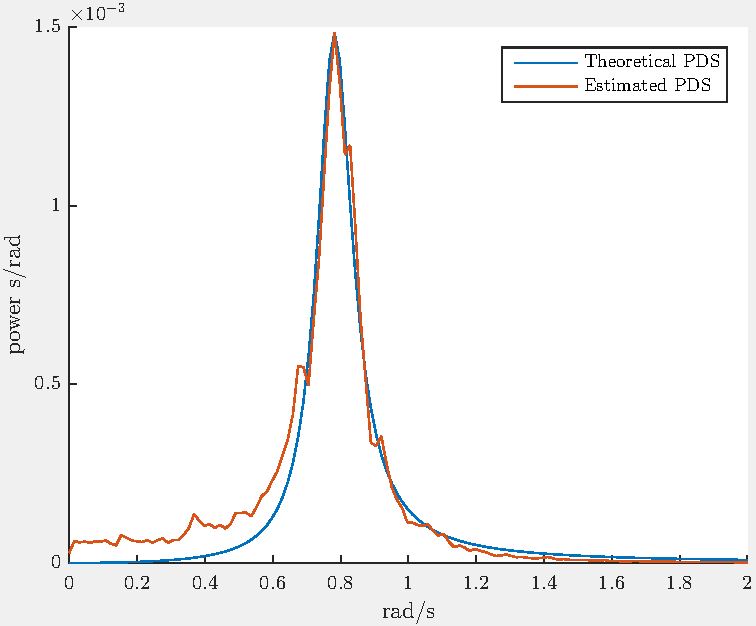
\includegraphics[width=0.5\textwidth]{images/2d-fitted_theoretical_PSD_vs_estimated_PSD}
    \caption{Fitted theoretical PSD vs estimated PSD}
    \label{fig:2d-fitted_theoretical_PSD_vs_estimated_PSD}
\end{figure}
